\documentclass{article}
\usepackage[a4paper,margin=2cm]{geometry} % <-- ajuste ici si tu veux plus de marge
\usepackage[french]{babel}
\addto\captionsfrench{\def\tablename{Tableau}}
\usepackage{amsmath}
\usepackage{amsfonts}
\usepackage{amsthm}
\usepackage{amssymb}
\usepackage{subfig}
\usepackage{cancel}
\usepackage{enumitem}
\usepackage{parskip}
\usepackage{pifont}
\usepackage[T1]{fontenc}
\usepackage[utf8]{inputenc}
\renewcommand\CancelColor{\color{red}}
\usepackage[dvipsnames]{xcolor}
\newcommand{\abs}[1]{\lvert #1 \rvert}
\newcommand{\tg}[1]{\textcolor{Green}{\quad\longleftarrow\text{#1}}}
\newcommand{\defn}[1]{\textcolor{Mulberry}{#1}}
\usepackage{graphicx}
\theoremstyle{plain}
\newtheorem{theorem}{Théorème}
\theoremstyle{definition}
\newtheorem{definition}{D\'{e}finition}
\newtheorem*{notation}{Notation}
\newtheorem{example}{Exemple}
\newtheorem*{property}{Propriété}
\newtheorem*{exercise}{Exercice}
\newtheorem*{remark}{Remarque}
\newtheorem*{note}{Note}
\newcounter{quCounter}
\newcommand\showQuCounter{\stepcounter{quCounter}\arabic{quCounter}}
\newcommand{\qu}{\paragraph{} \textbf{Question \showQuCounter : }}


\usepackage[normalem]{ulem} % pour \uline (soulignement)
\newcommand{\pk}[1]{\uline{#1}} % clé primaire soulignée
\newcommand{\fk}[1]{\#\uline{#1}} % clé étrangère + soulignée si elle est dans la PK
\newcommand{\fka}[1]{\##1} % clé étrangère (pas dans la PK)

\usepackage{fancyhdr}
\usepackage{multicol}
\usepackage{algpseudocode}
\usepackage{algorithm}
\fancypagestyle{plain}{
  \fancyhead[R]{\textbf{Hiver 2026}}
  \fancyhead[L]{\textbf{IFT 2935}}
  \renewcommand{\headrulewidth}{0pt}
}

\title{\textbf{Gestion d'un système de vente conditionnelle} \\
\large \textbf{Base de données}}
\author{Mamour Ndiaye 20257780, Jacob Déry 20248098, Yasin Patel 20306953, \\ Pierre Emery 20278920}
\date{\today}

\begin{document}

\maketitle
\thispagestyle{plain}

\noindent\makebox[\linewidth]{\rule{\linewidth}{0.6pt}}

\section*{Représentation Entité-Association de la base relationnelle}

\subsection*{Modèle E-A}
\begin{figure}[h]
    \centering
    \includegraphics[width=1\textwidth]{modele_ea.png}
    \caption{Modèle Entité-Association — Système de vente conditionnelle}
    \label{fig:modele_ea}
\end{figure}

\begin{figure}[h]
    \centering
    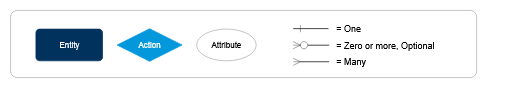
\includegraphics[width=0.4\textwidth]{legende_cardinalite.png}
    \caption{Légende des cardinalités}
    \label{fig:legende}
\end{figure}

\subsection*{Justification des éléments du modèle}
 
Le diagramme ci-dessus se suffit largement à lui-même; cette section
commente uniquement les choix de modélisation qui méritent une
explication.
 
\paragraph{Spécialisation d'\texttt{UTILISATEUR}.}
\texttt{ACHETEUR}, \texttt{ANNONCEUR} et \texttt{EXPERT} héritent tous
d'\texttt{UTILISATEUR} et n'ajoutent aucun attribut propre. Les données
personnelles (nom, prénom, courriel, mot de passe) sont ainsi centralisées
dans une seule table, et chaque rôle est distingué par sa simple
appartenance à la sous-entité correspondante. Les trois rôles sont
disjoints dans les données fournies mais le modèle permet techniquement
qu'un même utilisateur cumule plusieurs rôles.
 
\paragraph{\texttt{ESTIMATION} comme entité à part entière.}
L'estimation aurait pu être représentée comme un simple attribut du
produit. Nous l'avons promue en entité parce qu'elle possède un cycle de
vie propre (création par l'expert, puis validation ou rejet par
l'annonceur), un auteur distinct, et qu'un même produit peut en recevoir
plusieurs successivement. Son prix n'est jamais exposé aux acheteurs,
conformément à l'énoncé.
 
\paragraph{\texttt{OFFRE} comme entité plutôt qu'association.}
Une offre dépend toujours d'un acheteur et d'un produit, mais elle porte
ses propres attributs (\texttt{prix\_propose}, \texttt{date\_proposition})
et doit pouvoir être interrogée indépendamment des deux parties. Nous en
faisons donc une entité reliée à \texttt{PRODUIT} par \texttt{concerne} et
à \texttt{ACHETEUR} par \texttt{propose}.
 
\paragraph{Associations porteuses d'attributs.}
L'association \texttt{valide} porte l'attribut \texttt{decision}
(\texttt{en\_attente}, \texttt{valide} ou \texttt{rejete}), et
\texttt{propose} porte \texttt{date\_proposition}. Ces attributs
appartiennent à l'acte de validation ou de proposition plutôt qu'aux
entités qu'ils relient, ce qui justifie leur placement sur l'association.
 
\paragraph{Cardinalités notables.}
Un annonceur peut soumettre plusieurs produits (\texttt{precise}), un
expert peut réaliser plusieurs estimations (\texttt{estime}), un produit
peut recevoir plusieurs estimations successives et plusieurs offres
simultanées. Toutes les autres associations sont de type
« plusieurs côté entité faible, un côté entité forte ».
 
\paragraph{Contraintes d'intégrité métier.}
Trois règles encadrent le fonctionnement du système et sont garanties
par la couche applicative :
\begin{itemize}
    \item \textbf{Publication conditionnelle :} un produit n'est visible
    aux acheteurs que si au moins une de ses estimations est en état
    \texttt{valide}.
    \item \textbf{Vente automatique :} une offre dont le
    \texttt{prix\_propose} atteint ou dépasse le \texttt{prix\_estimation}
    validé déclenche immédiatement la conclusion de la vente.
    \item \textbf{Confidentialité du prix estimé :} le prix de
    l'estimation n'est jamais exposé côté acheteur; seul le
    \texttt{prix\_souhaite} est visible.
\end{itemize}
 

\pagebreak
\section*{Schéma relationnel}
Le modèle relationnel correspondant au diagramme Entité/Association est donné par
la liste de relations suivante :
\begin{itemize}
    \item \textbf{UTILISATEUR}(\pk{id}, nom, prenom, courriel, mot\_de\_passe)

    \item \textbf{ACHETEUR}({\fk{id\_utilisateur}})

    \item \textbf{ANNONCEUR}({\fk{id\_utilisateur}})

    \item \textbf{EXPERT}({\fk{id\_utilisateur}})

    \item \textbf{PRODUIT}(\pk{id\_produit}, nom\_produit, description, etat,
    prix\_souhaite, \fk{id\_annonceur})

    \item \textbf{ESTIMATION}(\pk{id\_estimation}, prix\_estimation, date\_estimation, \fk{id\_expert}, \fk{id\_produit})

    \item \textbf{VALIDE}({\fk{id\_annonceur}},{\fk{id\_estimation}},
    decision)

    \item \textbf{OFFRE}(\pk{id\_offre}, prix\_propose, \fk{id\_produit})

        
    \item \textbf{PROPOSE}(\fk{id\_offre}, \fk{id\_utilisateur}, date\_proposition)
\end{itemize}
\vspace{0.5cm}
\noindent
\textbf{À noter}
\vspace{0.2cm}

\noindent
Les conventions suivantes sont utilisées pour la présentation du modèle relationnel :
les clés primaires sont soulignées, les clés étrangères sont précédées du symbole
\texttt{\#} et lorsqu'une clé étrangère fait partie d'une clé primaire composée,
elle est à la fois précédée de \texttt{\#} et soulignée.

\vspace{0.3cm}
\noindent
Les entités \textbf{ACHETEUR}, \textbf{ANNONCEUR} et \textbf{EXPERT} sont des
spécialisations de \textbf{UTILISATEUR} : leur clé primaire est directement la clé
étrangère vers \textbf{UTILISATEUR}, ce qui garantit qu'aucun doublon d'information
de base (nom, courriel) n'est stocké.
L'association \textbf{VALIDE} entre \textbf{ANNONCEUR} et \textbf{ESTIMATION} est
matérialisée par une table de liaison car elle porte l'attribut \texttt{decision}.
L'association \textbf{ESTIME} entre \textbf{EXPERT} et \textbf{ESTIMATION} est
absorbée directement dans \textbf{ESTIMATION} via la clé étrangère
\texttt{id\_expert}, puisque chaque estimation appartient à exactement un expert.
De même, l'association \textbf{CONCERNE} entre \textbf{OFFRE} et \textbf{PRODUIT}
est absorbée dans \textbf{OFFRE} via \texttt{id\_produit}.

\section*{Explication des choix d'implémentation}
 
\subsection*{Choix des clés primaires}
 
Nous avons opté systématiquement pour des clés primaires artificielles
de type \texttt{SERIAL} plutôt que des clés naturelles. Plusieurs options
étaient envisageables pour identifier un utilisateur (courriel), un
produit (nom + annonceur + date) ou une offre (acheteur + produit +
date), mais chacune posait problème. Le courriel est modifiable par
l'utilisateur, ce qui forcerait une mise à jour en cascade dans les
quatre tables qui y réfèrent. Le couple (nom, annonceur) pour un produit
n'est pas unique : un même annonceur peut proposer deux iPhone 15. Bref, un
\texttt{SERIAL} contourne tous ces cas.
 
Pour les tables de liaison \texttt{Valide} et \texttt{propose}, nous
avons au contraire choisi des clés primaires \emph{composées} à partir
des clés étrangères (par exemple \texttt{(id\_annonceur, id\_estimation)}
pour \texttt{Valide}) la combinaison des deux FK est déjà unique
et porte la sémantique du lien donc ça semblait naturel ici.
 
\subsection*{Gestion des formats}
Nous avons choisi \texttt{DECIMAL(12,2)} plutôt
que \texttt{FLOAT} ou \texttt{REAL} pour tous les prix. Les types à
virgule flottante introduisent des erreurs d'arrondi
($0{,}1 + 0{,}2 \neq 0{,}3$ en binaire) qui sont inacceptables pour une
application financière où la comparaison entre un prix proposé et une
estimation déclenche une vente automatique. Le format \texttt{DECIMAL}
garantit une précision exacte au centime.
 
\subsection*{Duplications et séparations de tables}

\subsubsection*{Spécialisation d'\texttt{Utilisateur}.} 
Le modèle E-A décrit
\texttt{Acheteur}, \texttt{Annonceur} et \texttt{Expert} comme des
spécialisations d'\texttt{Utilisateur}. Nous trouvions que c'était une meilleure approche que tout fusionner dans \texttt{Utilisateur} avec des
colonnes booléennes \texttt{est\_acheteur}, \texttt{est\_annonceur},
\texttt{est\_expert} ou bien créer trois tables complètes qui dupliquent
nom, prénom, courriel, mot de passe. Nous avons donc préféré créer trois tables dont la
clé primaire est aussi une clé étrangère vers \texttt{Utilisateur}.
 
\begin{verbatim}
CREATE TABLE Acheteur (
    id_utilisateur INTEGER PRIMARY KEY
        REFERENCES Utilisateur(id) ON DELETE CASCADE
);
\end{verbatim}
 
L'option de tout fusionner rendait difficile d'attacher une contrainte d'intégrité
spécifique à un rôle (par exemple, seul un annonceur doit pouvoir être
référencé par \texttt{Produit.id\_annonceur}). L'option des tables complètes dupliquait
les données personnelles et créait un risque d'incohérence si un
utilisateur modifiait son courriel sous un rôle mais pas sous l'autre. L'option que nous avons choisies permet aux données personnelles de rester
uniques et un utilisateur peut cumuler plusieurs rôles simplement en
ayant une ligne dans plusieurs sous-tables.
 
\subsubsection*{Tables de liaison pour les associations porteuses d'attributs.}
Deux associations du modèle E-A portent leurs propres attributs :
\texttt{valide} (avec \texttt{decision}) et \texttt{propose} (avec
\texttt{date\_proposition}). Nous aurions pu absorber ces attributs
directement dans \texttt{Estimation} et \texttt{Offre} respectivement,
mais nous préferions les garder séparés puisque cela permet notamment qu'une
estimation existe temporairement sans décision (état \texttt{NULL} versus
\texttt{'en\_attente'}).
 
\subsubsection*{Absorption d'associations simples.} À l'inverse, les
associations \texttt{concerne} (\texttt{Offre} $\to$ \texttt{Produit}),
\texttt{precise} (\texttt{Produit} $\to$ \texttt{Annonceur}) et
\texttt{estime} / \texttt{pour} (\texttt{Estimation} $\to$ \texttt{Expert}
et \texttt{Produit}) ont été absorbées dans la table du côté
« plusieurs » sous forme de clés étrangères
(\texttt{id\_produit} dans \texttt{Offre},
\texttt{id\_annonceur} dans \texttt{Produit}, etc.).
Créer une table de liaison pour chacune aurait été gratuit en complexité
puisque ces associations ne portent pas d'attribut propre.

\pagebreak
\section*{Requêtes SQL et résultats attendus}
 
L'ensemble des requêtes qui suivent est rassemblé dans le fichier
\texttt{LMD.sql}.
 
\subsection*{Recherche d'un utilisateur par courriel}
 
\begin{verbatim}
SELECT * FROM Utilisateur WHERE courriel = ?;
\end{verbatim}
 
\noindent\textbf{Résultat :} la ligne de \texttt{Utilisateur} dont le
courriel correspond, ou aucune ligne si le courriel n'existe pas.
 
\subsection*{Recherche de produits par nom}
 
\begin{verbatim}
SELECT * FROM Produit
WHERE nom_produit LIKE CONCAT('%', ?, '%');
\end{verbatim}
 
\noindent\textbf{Résultat :} tous les produits dont le nom contient la
sous-chaîne passée en paramètre.
 
\subsection*{Recherche de produits par description}
 
\begin{verbatim}
SELECT * FROM Produit
WHERE description LIKE CONCAT('%', ?, '%');
\end{verbatim}
 
\noindent\textbf{Résultat :} tous les produits dont la description
contient la sous-chaîne passée en paramètre.
 
\subsection*{Recherche d'un produit par identifiant}
 
\begin{verbatim}
SELECT * FROM Produit WHERE id_produit = ?;
\end{verbatim}
 
\noindent\textbf{Résultat :} le produit correspondant à l'identifiant,
ou aucune ligne si l'identifiant n'existe pas.
 
\subsection*{Recherche de produits par fourchette de prix}
 
\begin{verbatim}
SELECT * FROM Produit
WHERE prix_souhaite BETWEEN ? AND ?;
\end{verbatim}
 
\noindent\textbf{Résultat :} tous les produits dont le prix souhaité se
situe dans la fourchette \texttt{[min, max]}, bornes incluses.
 
\subsection*{Recherche de produits par état}
 
\begin{verbatim}
SELECT Produit.*, Utilisateur.nom, Utilisateur.prenom
FROM Produit
JOIN Annonceur ON Produit.id_annonceur = Annonceur.id_utilisateur
JOIN Utilisateur ON Annonceur.id_utilisateur = Utilisateur.id
WHERE Produit.etat = ?;
\end{verbatim}
 
\noindent\textbf{Résultat :} tous les produits de l'état demandé
(\texttt{neuf}, \texttt{usage} ou \texttt{abime}), accompagnés du nom et
du prénom de leur annonceur.
 
\subsection*{Produits déposés par un annonceur}
 
\begin{verbatim}
SELECT Produit.*, Utilisateur.nom, Utilisateur.prenom
FROM Produit
JOIN Annonceur ON Produit.id_annonceur = Annonceur.id_utilisateur
JOIN Utilisateur ON Annonceur.id_utilisateur = Utilisateur.id
WHERE Produit.id_annonceur = ?;
\end{verbatim}
 
\noindent\textbf{Résultat :} tous les produits déposés par l'annonceur
identifié, avec son nom et son prénom.
 
\subsection*{Produits sans aucune offre}
 
\begin{verbatim}
SELECT Produit.*, Utilisateur.nom, Utilisateur.prenom
FROM Produit
JOIN Annonceur ON Produit.id_annonceur = Annonceur.id_utilisateur
JOIN Utilisateur ON Annonceur.id_utilisateur = Utilisateur.id
WHERE NOT EXISTS (
    SELECT 1 FROM Offre
    WHERE Offre.id_produit = Produit.id_produit
);
\end{verbatim}
 
\noindent\textbf{Résultat :} tous les produits n'ayant reçu aucune
offre, avec l'identité de leur annonceur.
 
\subsection*{Toutes les estimations sur un produit}
 
\begin{verbatim}
SELECT Estimation.*, Utilisateur.nom, Utilisateur.prenom, Valide.decision
FROM Estimation
JOIN Expert ON Estimation.id_expert = Expert.id_utilisateur
JOIN Utilisateur ON Expert.id_utilisateur = Utilisateur.id
LEFT JOIN Valide ON Estimation.id_estimation = Valide.id_estimation
WHERE Estimation.id_produit = ?;
\end{verbatim}
 
\noindent\textbf{Résultat :} toutes les estimations faites sur le
produit, avec l'expert correspondant et la décision de l'annonceur
(\texttt{NULL} si aucune décision n'a encore été prise).
 
\subsection*{Estimations validées sur un produit}
 
\begin{verbatim}
SELECT Estimation.*, Utilisateur.nom, Utilisateur.prenom
FROM Estimation
JOIN Expert ON Estimation.id_expert = Expert.id_utilisateur
JOIN Utilisateur ON Expert.id_utilisateur = Utilisateur.id
JOIN Valide ON Estimation.id_estimation = Valide.id_estimation
WHERE Estimation.id_produit = ? AND Valide.decision = 'valide';
\end{verbatim}
 
\noindent\textbf{Résultat :} uniquement les estimations validées par
l'annonceur pour le produit, avec l'expert correspondant.
 
\subsection*{Offres reçues sur un produit}
 
\begin{verbatim}
SELECT Offre.*, Utilisateur.nom, Utilisateur.prenom, propose.date_proposition
FROM Offre
JOIN propose ON Offre.id_offre = propose.id_offre
JOIN Acheteur ON propose.id_utilisateur = Acheteur.id_utilisateur
JOIN Utilisateur ON Acheteur.id_utilisateur = Utilisateur.id
WHERE Offre.id_produit = ?;
\end{verbatim}
 
\noindent\textbf{Résultat :} toutes les offres déposées sur le produit,
avec l'identité de l'acheteur et la date de proposition.
 
\subsection*{Offres soumises par un acheteur}
 
\begin{verbatim}
SELECT Offre.*, Produit.nom_produit, Produit.description,
       propose.date_proposition
FROM Offre
JOIN propose ON Offre.id_offre = propose.id_offre
JOIN Produit ON Offre.id_produit = Produit.id_produit
WHERE propose.id_utilisateur = ?;
\end{verbatim}
 
\noindent\textbf{Résultat :} toutes les offres soumises par l'acheteur
identifié, avec le nom et la description du produit concerné et la date
de proposition.
 
\subsection*{Offres des trente derniers jours}
 
\begin{verbatim}
SELECT Offre.*, Produit.nom_produit, Utilisateur.nom, Utilisateur.prenom,
       propose.date_proposition
FROM Offre
JOIN propose ON Offre.id_offre = propose.id_offre
JOIN Acheteur ON propose.id_utilisateur = Acheteur.id_utilisateur
JOIN Utilisateur ON Acheteur.id_utilisateur = Utilisateur.id
JOIN Produit ON Offre.id_produit = Produit.id_produit
WHERE propose.date_proposition >= CURRENT_DATE - INTERVAL '30 days'
ORDER BY propose.date_proposition DESC;
\end{verbatim}
 
\noindent\textbf{Résultat :} toutes les offres soumises au cours des
trente derniers jours, triées de la plus récente à la plus ancienne,
avec le produit et l'acheteur concernés.
 
\subsection*{Fiche détaillée d'une offre}
 
\begin{verbatim}
SELECT Offre.*, Produit.nom_produit, Produit.description,
       Produit.etat, Produit.prix_souhaite,
       U_Acheteur.nom AS acheteur_nom, U_Acheteur.prenom AS acheteur_prenom,
       U_Annonceur.nom AS annonceur_nom, U_Annonceur.prenom AS annonceur_prenom,
       propose.date_proposition
FROM Offre
JOIN Produit ON Offre.id_produit = Produit.id_produit
JOIN Annonceur ON Produit.id_annonceur = Annonceur.id_utilisateur
JOIN Utilisateur U_Annonceur ON Annonceur.id_utilisateur = U_Annonceur.id
JOIN propose ON Offre.id_offre = propose.id_offre
JOIN Acheteur ON propose.id_utilisateur = Acheteur.id_utilisateur
JOIN Utilisateur U_Acheteur ON Acheteur.id_utilisateur = U_Acheteur.id
WHERE Offre.id_offre = ?;
\end{verbatim}
 
\noindent\textbf{Résultat :} une seule ligne rassemblant toutes les
informations contextuelles d'une offre : détails du produit, identité de
l'acheteur, identité de l'annonceur et date de proposition.
 
\subsection*{Vérification de la conclusion d'une vente}
 
\begin{verbatim}
SELECT
    CASE
        WHEN prix_souhaite IS NOT NULL AND ? <  prix_souhaite THEN 'REFUSE'
        WHEN prix_souhaite IS NOT NULL AND ? >= prix_souhaite THEN 'ACCEPT'
        ELSE 'PENDING'
    END AS decision
FROM Produit
WHERE id_produit = ?;
\end{verbatim}
 
\noindent\textbf{Résultat :} \texttt{'ACCEPT'} si le prix proposé
atteint ou dépasse le prix souhaité du produit, \texttt{'REFUSE'} sinon.
 
\subsection*{Statistiques de performance des experts}
 
\begin{verbatim}
SELECT U_Expert.nom, U_Expert.prenom,
       SUM(Estimation.prix_estimation) AS total_estime,
       COUNT(Estimation.id_estimation) AS nb_estimation
FROM Expert
JOIN Utilisateur AS U_Expert ON Expert.id_utilisateur = U_Expert.id
JOIN Estimation ON U_Expert.id_utilisateur = Estimation.id_expert
JOIN Valide ON Estimation.id_estimation = Valide.id_estimation
WHERE Valide.decision = 'valide'
GROUP BY U_Expert.nom, U_Expert.prenom
HAVING COUNT(Estimation.id_estimation) > 1
ORDER BY total_estime DESC;
\end{verbatim}
 
\noindent\textbf{Résultat :} une ligne par expert ayant produit plus
d'une estimation validée, indiquant le montant total estimé et le nombre
d'estimations, triée du plus gros volume au plus faible.
 
\subsection*{Consultation des prix validés}
 
\begin{verbatim}
SELECT U_Annonceur.nom AS nom_annonceur, Produit.nom_produit,
       U_Expert.nom AS nom_expert, Estimation.prix_estimation
FROM Annonceur
JOIN Utilisateur U_Annonceur ON Annonceur.id_utilisateur = U_Annonceur.id
JOIN Produit ON Annonceur.id_utilisateur = Produit.id_annonceur
JOIN Estimation ON Estimation.id_produit = Produit.id_produit
JOIN Expert ON Estimation.id_expert = Expert.id_utilisateur
JOIN Utilisateur U_Expert ON Expert.id_utilisateur = U_Expert.id
JOIN Valide ON Valide.id_estimation = Estimation.id_estimation
          AND Valide.id_annonceur = Produit.id_annonceur
WHERE Valide.decision = 'valide';
\end{verbatim}
 
\noindent\textbf{Résultat :} pour chaque estimation validée, le nom de
l'annonceur, le nom du produit, le nom de l'expert et le prix
d'estimation officiel.

\subsection*{Produits visibles aux acheteurs}

\begin{verbatim}
SELECT DISTINCT Produit.*
FROM Produit
JOIN Estimation ON Estimation.id_produit = Produit.id_produit
JOIN Valide ON Valide.id_estimation = Estimation.id_estimation
WHERE Valide.decision = 'valide';
\end{verbatim}

\noindent\textbf{Résultat :} tous les produits dont au moins une
estimation a été validée par l'annonceur, donc visibles aux acheteurs.

\subsection*{Recherche d'une estimation en attente de décision}

\begin{verbatim}
SELECT Estimation.id_estimation
FROM Estimation
JOIN Valide ON Valide.id_estimation = Estimation.id_estimation
WHERE Estimation.id_produit = ?
  AND Valide.id_annonceur = ?
  AND Valide.decision = 'en_attente'
LIMIT 1;
\end{verbatim}

\noindent\textbf{Résultat :} l'identifiant d'une estimation du produit
demandé pour laquelle l'annonceur n'a pas encore pris de décision, ou
aucune ligne si toutes les estimations ont déjà été traitées.

\pagebreak
\section*{Guide d'utilisateur de l'application}

Ce mini-guide suit un utilisateur typique à travers les deux interfaces de l'application : d'abord l'acheteur, puis l'annonceur.

\subsection*{Installation et lancement}
 
Avant d'utiliser l'application, quelques étapes de configuration sont nécessaires.
 
\paragraph{Configuration JDBC.}
Renommer un fichier en \texttt{db.properties} à la racine du projet, puis ajuster les valeurs pour qu'elles correspondent à l'environnement local :
 
\begin{verbatim}
url=jdbc:postgresql://localhost:5432/IFT2935_Projet
user=postgres
password=mot_de_passe
\end{verbatim}
 
L'hôte et le port par défaut sont \texttt{localhost:5432}; si l'instance PostgreSQL utilise un autre port, il faut ajuster l'URL en conséquence. Le nom de la base (\texttt{IFT2935\_Projet} par défaut) doit correspondre exactement à celle créée avec \texttt{DDL.sql}. L'utilisateur est généralement \texttt{postgres}; le mot de passe est celui défini lors de l'installation de PostgreSQL.
 
\paragraph{Compilation.}
Depuis la racine du projet :
 
\begin{verbatim}
javac -d src -cp "lib/postgresql-42.7.2.jar" src/*.java
\end{verbatim}
 
\paragraph{Lancement.}
Depuis la racine du projet :
 
\begin{verbatim}
java -cp "src;lib/postgresql-42.7.2.jar;." Main
\end{verbatim}
 
\paragraph{Comptes de test.}
Une fois l'application lancée, les comptes suivants, préconfigurés dans \texttt{LMD.sql}, permettent de tester chaque rôle :
 
\begin{center}
\begin{tabular}{lll}
\textbf{Rôle} & \textbf{Courriel} & \textbf{Mot de passe} \\
\hline
Acheteur  & \texttt{prof.acheteur@test.com}  & \texttt{test} \\
Annonceur & \texttt{prof.annonceur@test.com} & \texttt{test} \\
\end{tabular}
\end{center}
\subsection*{Connexion}

L'application s'ouvre sur un écran de connexion commun à tous les rôles. L'utilisateur entre son courriel et son mot de passe, et l'application détermine automatiquement son rôle (acheteur, annonceur ou expert) pour afficher l'interface appropriée.

\begin{figure}[H]
    \centering
    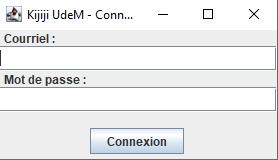
\includegraphics[width=0.3\linewidth]{login.png}
    \caption{Écran de connexion initial.}
    \label{fig:login}
\end{figure}

En cas de courriel ou de mot de passe invalide, un message d'erreur informe l'utilisateur sans révéler lequel des deux champs est incorrect (bonne pratique de sécurité).

\begin{figure}[H]
    \centering
    
\includegraphics[width=0.3\linewidth]{courriel_invalide.png}
    \caption{Message d'erreur lorsque les identifiants sont invalides.}
    \label{fig:courriel-invalide}
\end{figure}

\subsection*{Interface acheteur}

Une fois connecté avec un compte acheteur, l'utilisateur voit la liste complète des produits dont l'estimation a été validée par leur annonceur. Seuls ces produits sont visibles, conformément à la logique métier.

\begin{figure}[H]
    \centering
    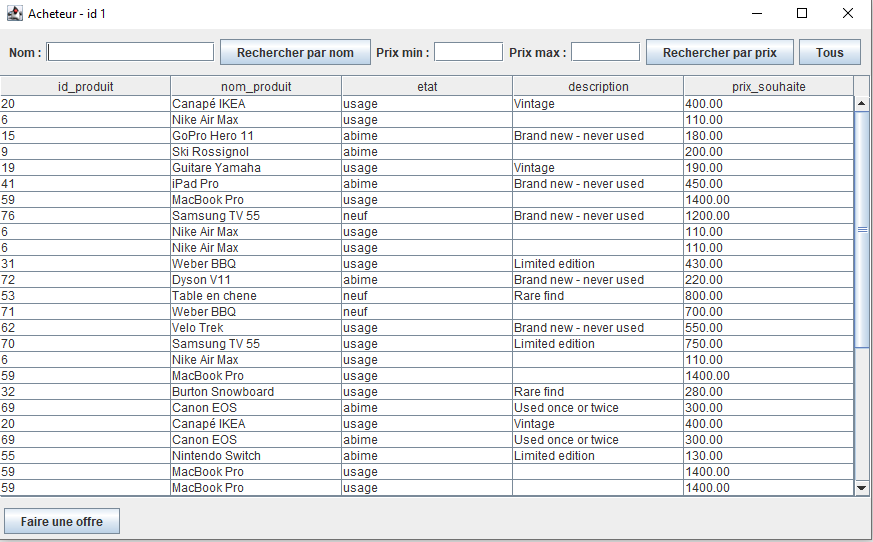
\includegraphics[width=1\linewidth]{acheteur.png}
    \caption{Page d'accueil acheteur : liste des produits disponibles.}
    \label{fig:acheteur}
\end{figure}

L'acheteur peut filtrer la liste par nom de produit...

\begin{figure}[H]
    \centering
    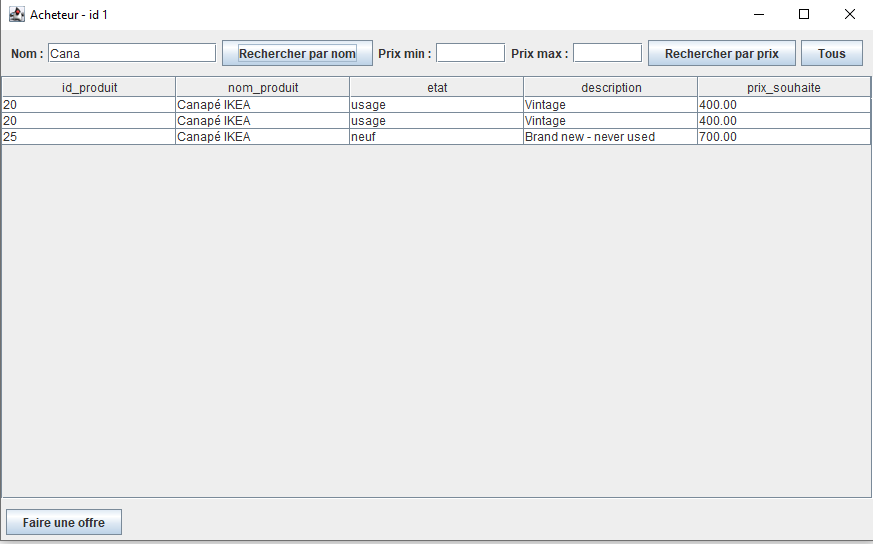
\includegraphics[width=1\linewidth]{recherche_noms.png}
    \caption{Recherche par nom : les résultats sont filtrés selon la sous-chaîne saisie.}
    \label{fig:recherche-noms}
\end{figure}

...ou par fourchette de prix.

\begin{figure}[H]
    \centering
    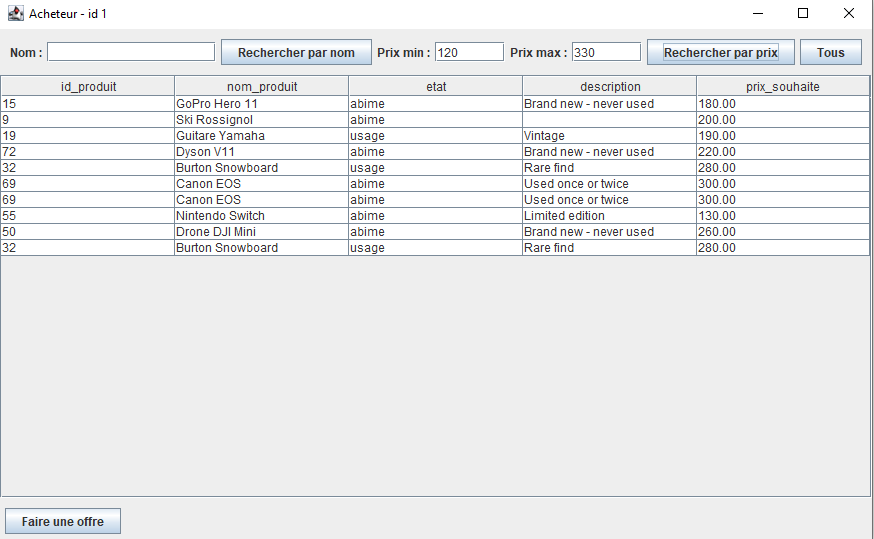
\includegraphics[width=1\linewidth]{recherche_prix.png}
    \caption{Recherche par intervalle de prix souhaité.}
    \label{fig:recherche-prix}
\end{figure}

Les entrées non numériques dans les champs de prix sont rejetées avec un message d'erreur.

\begin{figure}[H]
    \centering
    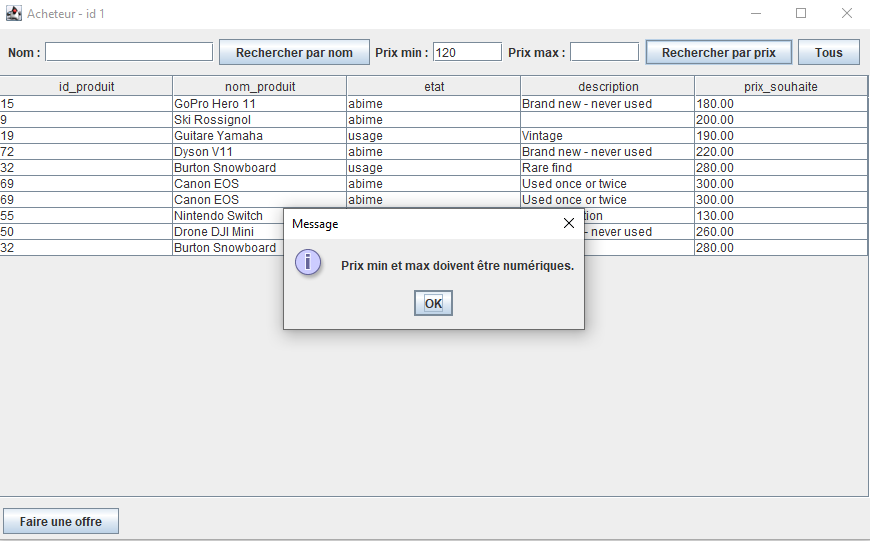
\includegraphics[width=1\linewidth]{erreur_prix_invalide.png}
    \caption{Validation des entrées : un prix non numérique est refusé.}
    \label{fig:erreur-prix-invalide}
\end{figure}

Pour faire une offre, l'acheteur sélectionne d'abord une ligne dans le tableau...

\begin{figure}[H]
    \centering
    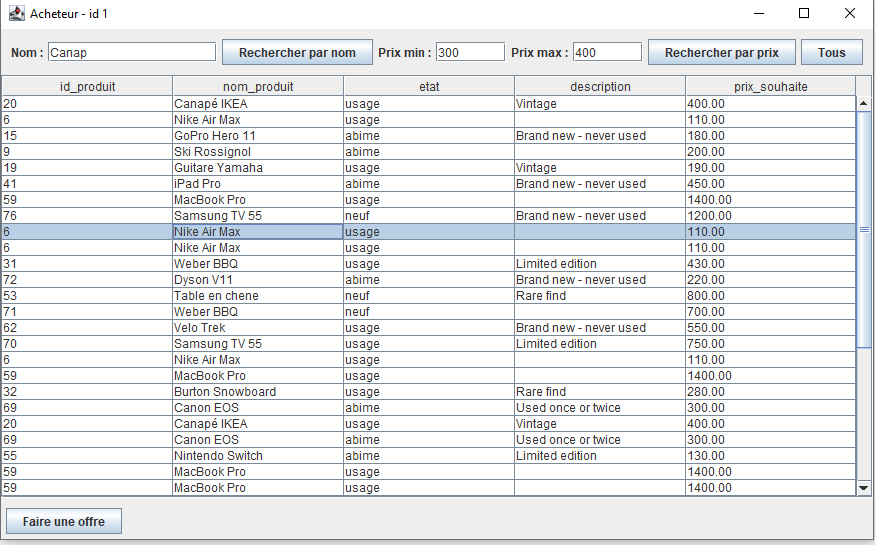
\includegraphics[width=1\linewidth]{selection_produit.png}
    \caption{Sélection d'un produit dans la liste.}
    \label{fig:selection-produit}
\end{figure}

...puis clique sur le bouton « Faire une offre ».

\begin{figure}[H]
    \centering
    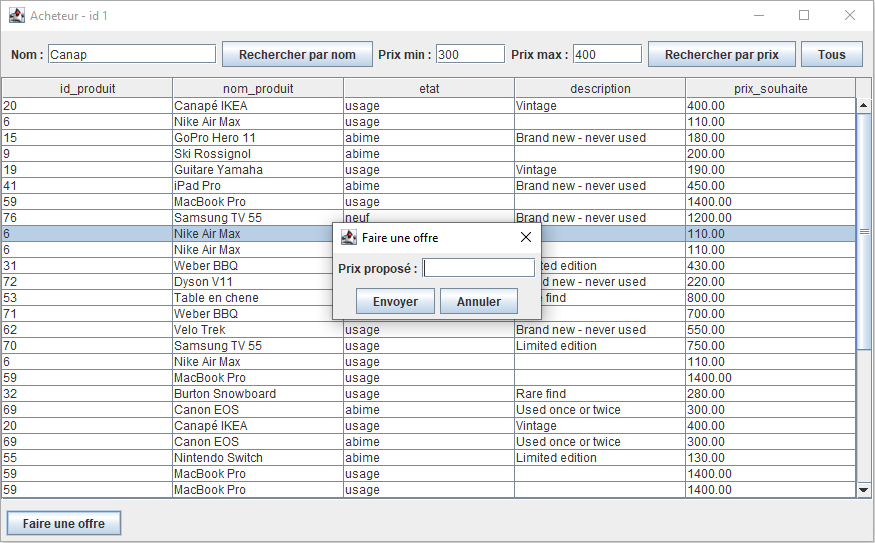
\includegraphics[width=1\linewidth]{boutton_offre.png}
    \caption{Bouton « Faire une offre » disponible en bas de l'écran.}
    \label{fig:bouton-offre}
\end{figure}

Une fenêtre s'ouvre pour saisir le prix proposé. Si l'offre atteint ou dépasse l'estimation (invisible pour l'acheteur), la vente est automatiquement conclue.

\begin{figure}[H]
    \centering
    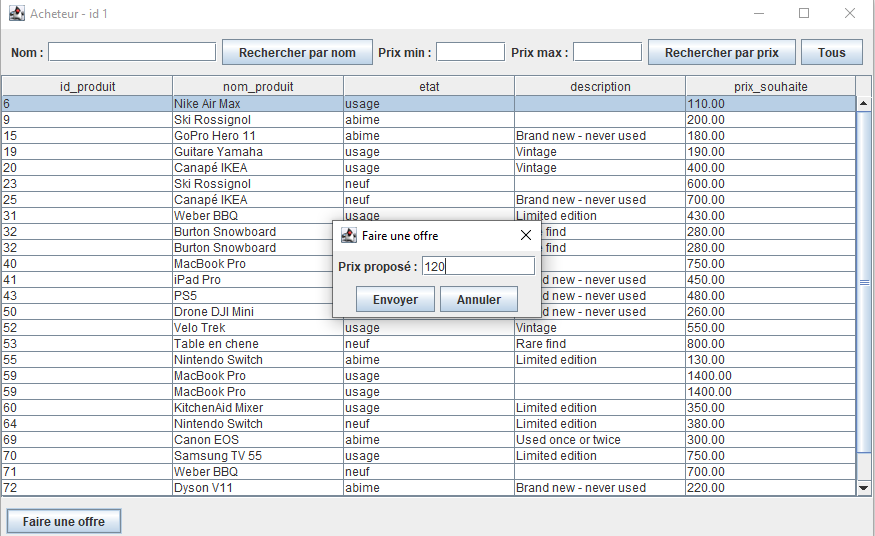
\includegraphics[width=1\linewidth]{prix_propose.png}
    \caption{Prix proposé plus grand que le prix souhaité}
    \label{fig:placeholder}
\end{figure}

\begin{figure}[H]
    \centering
    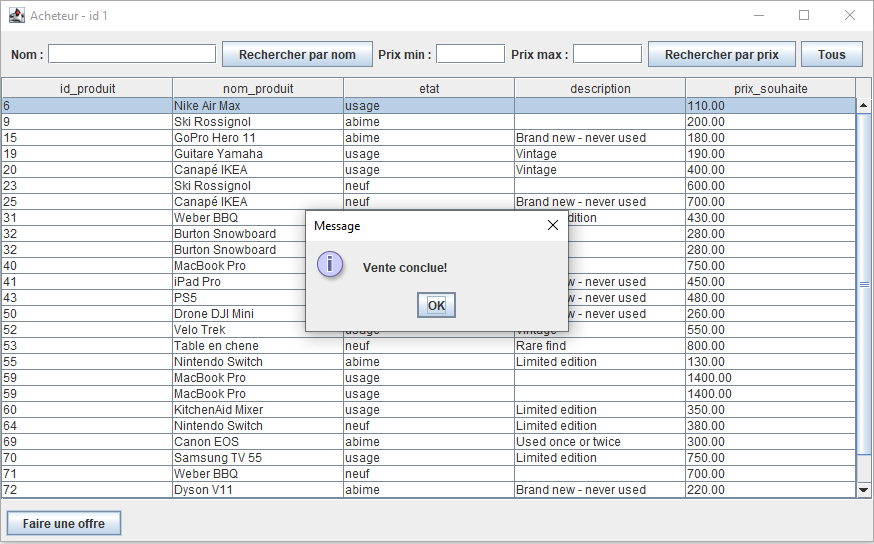
\includegraphics[width=1\linewidth]{vente_conclue.png}
    \caption{Vente Conclue}
    \label{fig:placeholder}
\end{figure}

Et puis si le prix est plus bas que le prix souhaité alors l'offre est simplement enregistrée sans que la transaction soit immédiatement conclue.
\begin{figure}[H]
    \centering
    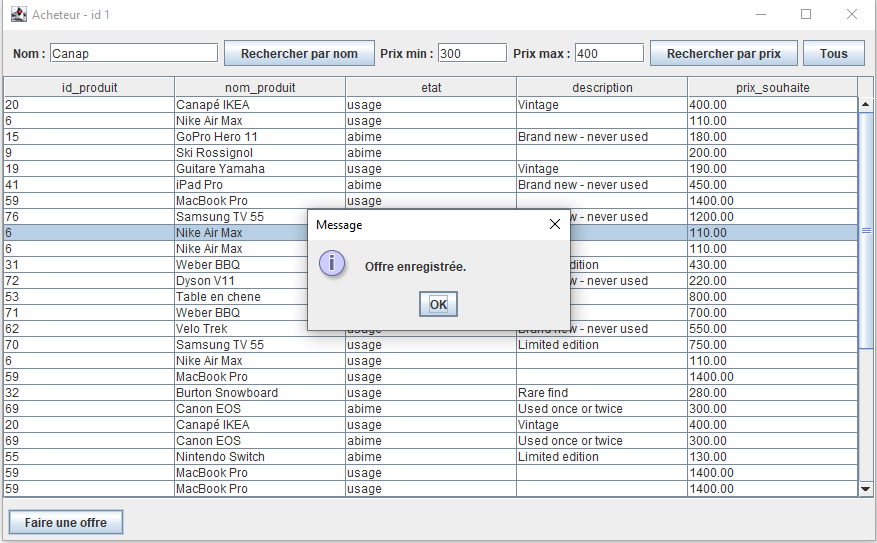
\includegraphics[width=1\linewidth]{proposition_offre.png}
    \caption{Saisie du prix proposé pour le produit sélectionné.}
    \label{fig:proposition-offre}
\end{figure}

D'autres cas limites sont également gérés. Une recherche sans résultat retourne une liste vide...

\begin{figure}[H]
    \centering
    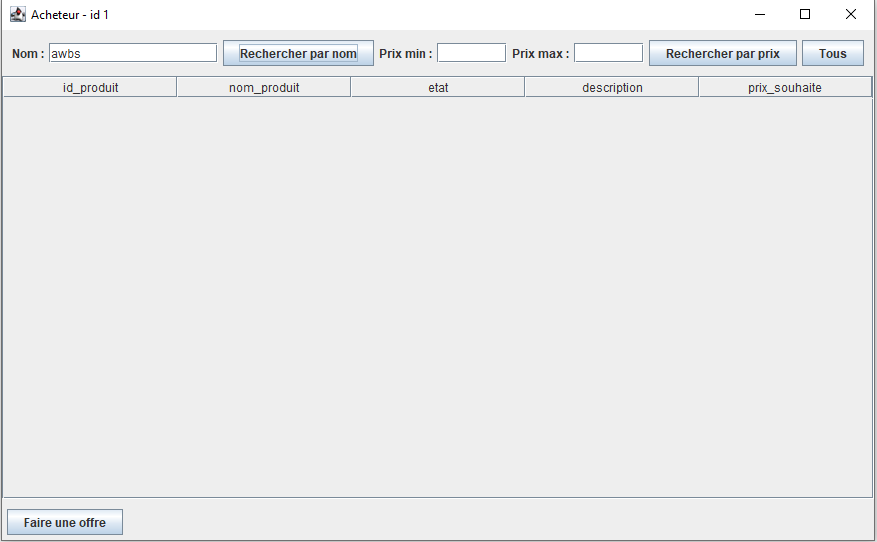
\includegraphics[width=1\linewidth]{recherche_nom_existepas.png}
    \caption{Recherche par nom sans correspondance : aucun résultat affiché.}
    \label{fig:recherche-nom-inexistant}
\end{figure}

...et une fourchette de prix incohérente (maximum inférieur au minimum) retourne également une liste vide sans provoquer d'erreur.

\begin{figure}[H]
    \centering
    \includegraphics[width=1\linewidth]{recherche_prix_max<min.png}
    \caption{Recherche avec un prix maximum inférieur au minimum : aucun résultat.}
    \label{fig:recherche-prix-incoherent}
\end{figure}

\subsection*{Interface annonceur}

En se connectant avec un compte annonceur, l'utilisateur accède à un onglet présentant ses produits et leur statut de validation.

\begin{figure}[H]
    \centering
    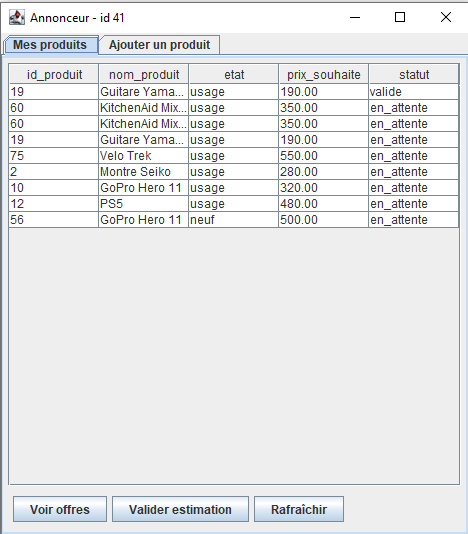
\includegraphics[width=0.5\linewidth]{annonceur.png}
    \caption{Onglet « Mes produits » : liste des produits de l'annonceur avec leur statut.}
    \label{fig:annonceur}
\end{figure}

L'onglet « Ajouter un produit » permet de soumettre une nouvelle annonce. L'annonceur renseigne le nom, l'état, une description et le prix souhaité.

\begin{figure}[H]
    \centering
    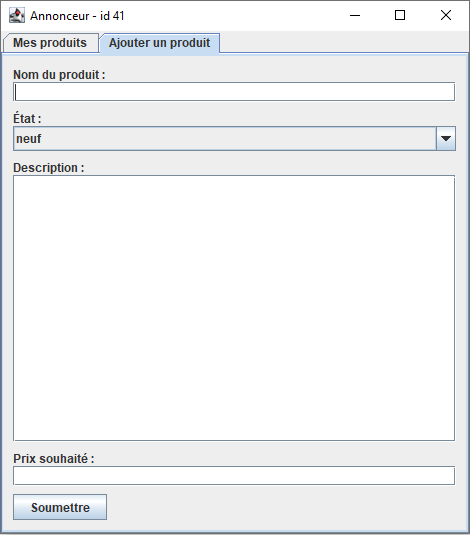
\includegraphics[width=0.5\linewidth]{ajouter_produit.png}
    \caption{Formulaire d'ajout d'un nouveau produit.}
    \label{fig:ajouter-produit}
\end{figure}

Dès la soumission, un expert (choisi aléatoirement) propose une estimation du prix. C'est le rôle de la fenêtre suivante, qui simule l'intervention de l'expert.

\begin{figure}[H]
    \centering
    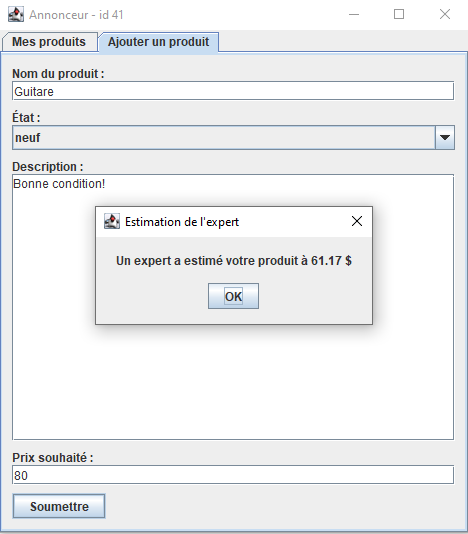
\includegraphics[width=0.5\linewidth]{une_fois_ajoute.png}
    \caption{Fenêtre d'estimation : l'expert communique son évaluation du prix.}
    \label{fig:estimation-expert}
\end{figure}

L'annonceur doit alors décider s'il accepte ou rejette cette estimation.

\begin{figure}[H]
    \centering
    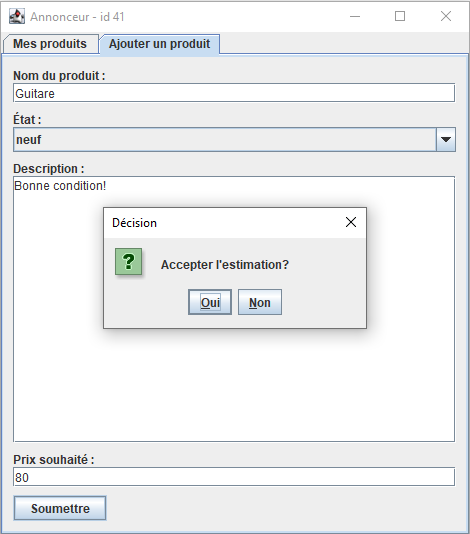
\includegraphics[width=0.5\linewidth]{accepter_estimation.png}
    \caption{Dialogue de décision : accepter ou refuser l'estimation de l'expert.}
    \label{fig:accepter-estimation}
\end{figure}

Dans ce premier scénario, l'annonceur refuse l'estimation : le produit est enregistré avec le statut \texttt{rejete} et ne sera pas visible aux acheteurs.

\begin{figure}[H]
    \centering
    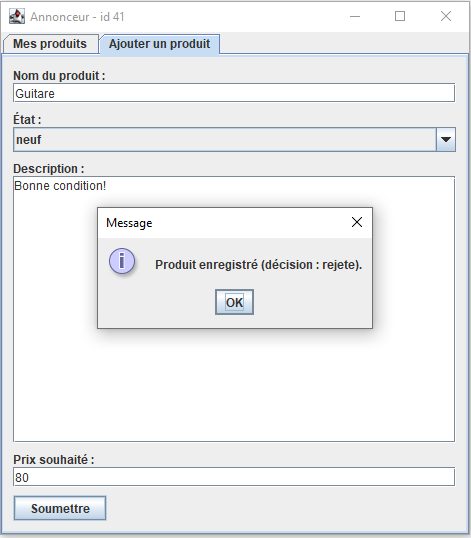
\includegraphics[width=0.5\linewidth]{rejetter.png}
    \caption{Confirmation : l'estimation est rejetée et le produit marqué comme tel.}
    \label{fig:rejetter}
\end{figure}

L'annonceur tente l'opération une seconde fois pour un autre produit ; une nouvelle estimation est générée.

\begin{figure}[H]
    \centering
    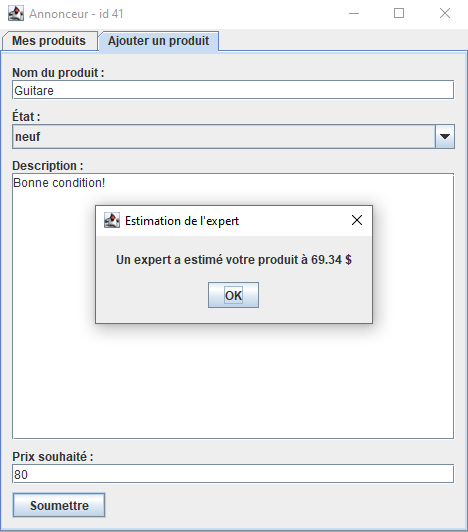
\includegraphics[width=0.5\linewidth]{autre_estimation.png}
    \caption{Nouvelle soumission : l'expert propose une seconde estimation.}
    \label{fig:autre-estimation}
\end{figure}

Cette fois, l'annonceur accepte l'estimation.

\begin{figure}[H]
    \centering
    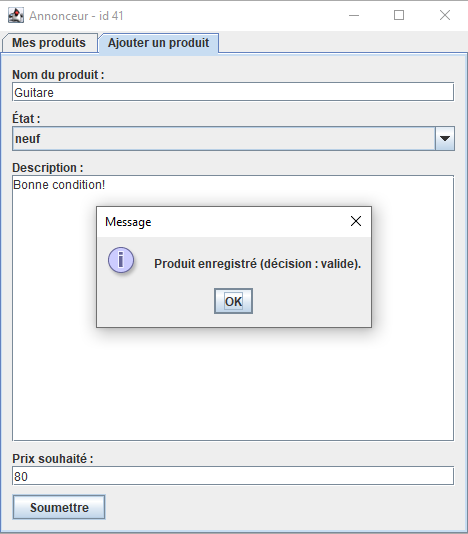
\includegraphics[width=0.5\linewidth]{accepter.png}
    \caption{L'annonceur accepte l'estimation de l'expert.}
    \label{fig:accepter}
\end{figure}

La liste « Mes produits » se met à jour pour refléter les deux nouveaux produits avec leurs statuts respectifs (\texttt{valide} et \texttt{rejete}).

\begin{figure}[H]
    \centering
    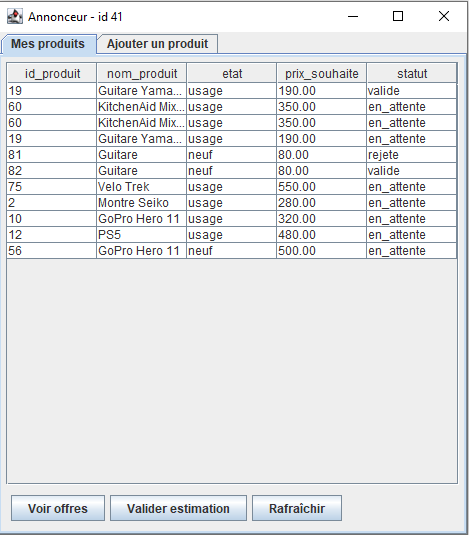
\includegraphics[width=0.5\linewidth]{mes_produits_update.png}
    \caption{Liste des produits actualisée après les deux soumissions.}
    \label{fig:mes-produits-update}
\end{figure}

\subsection*{Gestion des offres reçues et des estimations}

Pour un produit dont le statut est \texttt{valide}, l'annonceur peut consulter les offres reçues via le bouton « Voir offres ».

\begin{figure}[H]
    \centering
    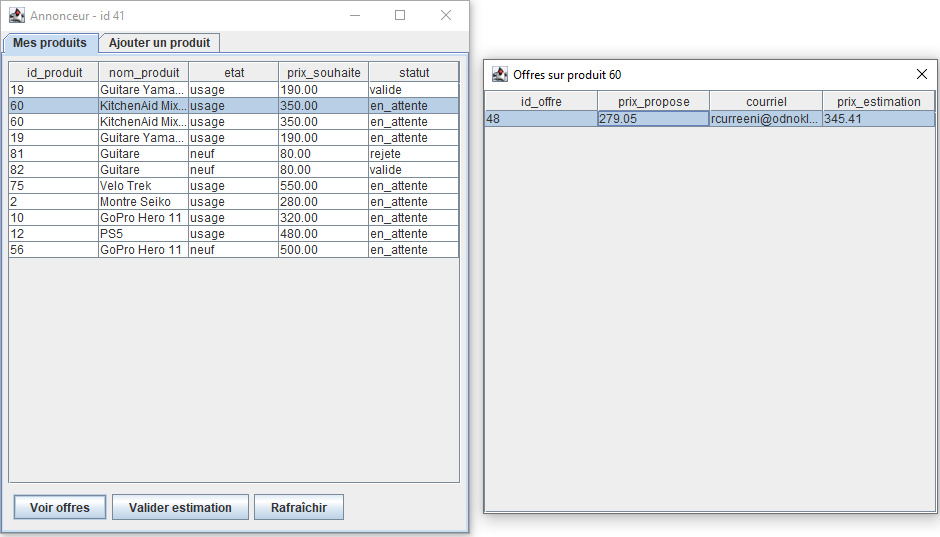
\includegraphics[width=0.8\linewidth]{bouton_voiroffres.png}
    \caption{Fenêtre des offres : prix proposés par les acheteurs, avec marqueur « VENDU » pour les offres atteignant l'estimation.}
    \label{fig:voir-offres}
\end{figure}

L'annonceur peut aussi retourner a posteriori sur une estimation encore en attente via le bouton « Valider estimation ». Si aucune estimation n'est en attente pour le produit sélectionné, un message l'indique.

\begin{figure}[H]
    \centering
    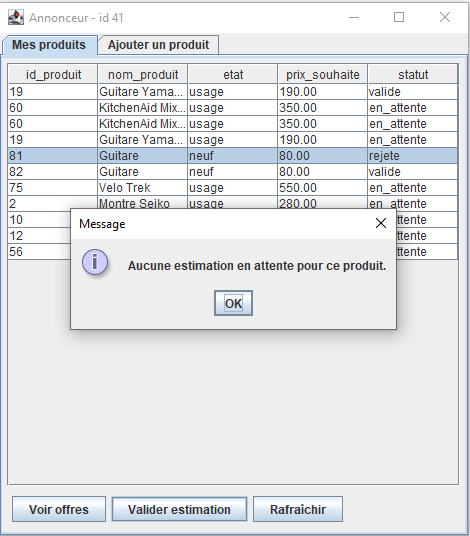
\includegraphics[width=0.5\linewidth]{aucune_estimation.png}
    \caption{Aucune estimation en attente pour le produit sélectionné.}
    \label{fig:aucune-estimation}
\end{figure}

Sinon, la fenêtre de décision s'affiche à nouveau.

\begin{figure}[H]
    \centering
    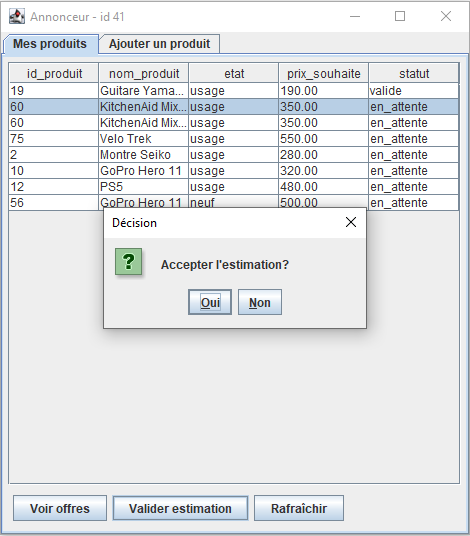
\includegraphics[width=0.5\linewidth]{bouton_valider_estimation.png}
    \caption{Validation différée : décision demandée pour une estimation en attente.}
    \label{fig:valider-estimation}
\end{figure}

Selon le choix, le produit bascule en statut \texttt{rejete}...

\begin{figure}[H]
    \centering
    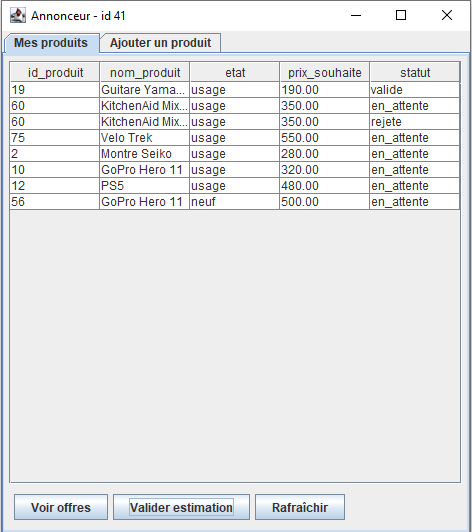
\includegraphics[width=0.5\linewidth]{refus.png}
    \caption{L'estimation en attente est refusée.}
    \label{fig:refus}
\end{figure}

...ou en statut \texttt{valide}, ce qui le rend aussitôt visible aux acheteurs.

\begin{figure}[H]
    \centering
    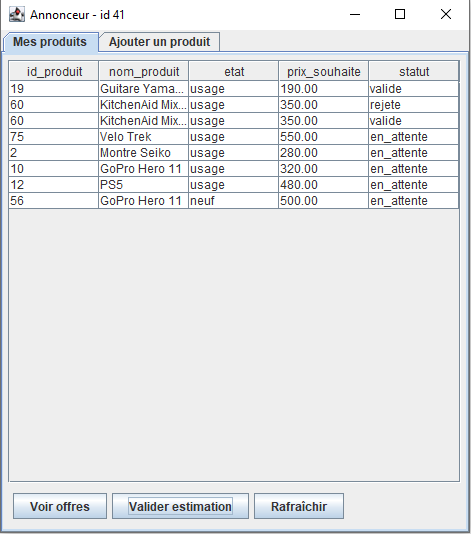
\includegraphics[width=0.5\linewidth]{accept.png}
    \caption{L'estimation en attente est acceptée : le produit devient disponible à la vente.}
    \label{fig:accept}
\end{figure}

\end{document}